% ╒══════════════════════════════════════════════════════════════════════════╕ %
% │                                TITLE PAGE                                │ %
% ╘══════════════════════════════════════════════════════════════════════════╛ %

\begin{titlepage}
    \begin{onecolumn}
        \begin{center}
            {\Huge \booktitle}
            
            \vspace{0.5cm}
            
\includegraphics[width=\textwidth]{images/hr.png}
            
            \vspace{0.5cm}
            {\huge \booksubtitle}
            
            \vspace{0.5cm}

            % Replace this picture with cover art
            % \begin{picture}(500,200)
            %     \put(0,0){\framebox(500,200)}
            % \end{picture}
            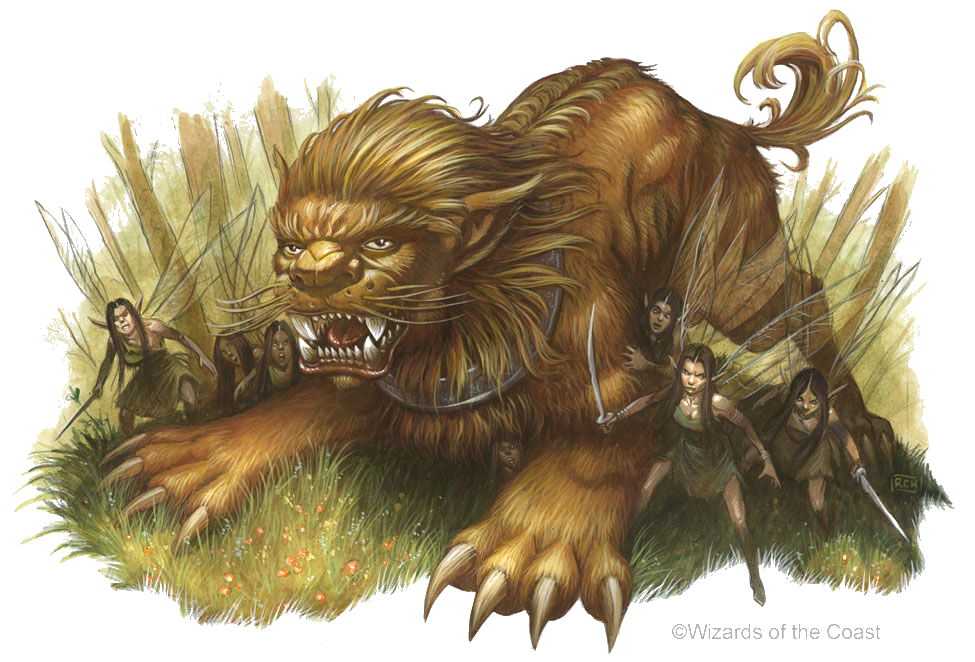
\includegraphics[width=\textwidth]{images/foo.png}
            
            \vspace{0.5cm}
            \lipsum[1] % Put the description here
            
            \vspace{0.5cm}
            {\Large A xx-hour adventure for x xxth--xxth level characters}

            
            \vfill
            {\Large by \bookauthor}
            
            % \vfill
        \end{center}


        \begin{minipage}{0.94\textwidth}
            {%
            \setlength\intextsep{0pt}
            \begin{wrapfigure}[11]{l}{0.188\textwidth}
                \centering
                
\includegraphics[width=\linewidth]{images/dmsguild.jpg}  
                    \end{wrapfigure}
            {\footnotesize
                DUNGEONS \& DRAGONS, D\&D, Wizards of the Coast, Forgotten Realms, Ravenloft, the dragon ampersand, and all other Wizards of the Coast product names, and their respective logos are trademarks of Wizards of the Coast in the USA and other countries.\\
                This work contains material that is copyright Wizards of the Coast and/or other authors. Such material is used with permission under the Community Content Agreement for Dungeon Masters Guild.\\
                All other original material in this work is copyright 2016 by \bookauthor\ and published under the Community Content Agreement for Dungeon Masters Guild.\\}
            }
        \end{minipage}
    \end{onecolumn}
\end{titlepage}
\clearpage

\setcounter{tocdepth}{2} %Tablle of contents depth
\tableofcontents